\chapter{\label{ch:3}Measuring nucleotide binding to K\ATP} 

\graphicspath{{figures/ch3/}}

\minitoc

\section{Designing a nucleotide binding assay}

\subsection{Criteria for a useful assay}

Previous approaches to measuring nucleotide binding directly have relied on isolating binding to individual classes of site by disrupting protein function; either by introducing mutations which abolish binding to a particular site or by measuring binding to Kir6.2 or SUR1 alone.
Traditionally, assays such as radioligand binding experiments require purifying the protein out of it's native membrane environment, thus rendering the channels nonfunctional.

To improve on these methods, an ideal assay measuring nucleotide binding to the K\ATP{} channel neeeds to fulfill a number of criteria.

\begin{enumerate}
	\item We need sufficient spatial sensitivity to distinguish between different classes of binding site; i.e. the assay should be capable of distingushing binding to Kir6.2 from binding to NBS1 or NBS2.
	\item We should be able to measure binding to a functional channel, for which we need to be able to measure binding in a membrane.
	\item There should be minimal perturbation of the channel in order for binding measurements to be physiologically relevant.
\end{enumerate}

TO fulfill these criteria, we used an approach involving a fluorescent unnatural amino acid, ANAP.
ANAP has been used increasing widely in the study of ion channel structure and function due to a few desirable qualities.

\begin{enumerate}
	\item It is smaller than traditional fluorescent labels such as fluorescent proteins or rhodamine derivatives.
	Therefore, it should be less perturbing to the function of the protein it labels.
	\item As it is an amino acid, it can be site-specifically inserted into any protein.
	This avoids the issues of other small chemical dyes which are targeted to a site via post-translational covalent modifications, typically by reacting with a cysteine residue.
	While this can be avoided in some proteins by mutating each cysteine residue to an alternative residue to avoid off-target labelling, there are functionally important cysteines in the K\ATP{} channel which cannot be mutated.
	\item ANAP is environmentally sensitive, which has been used to great effect in other studies.
	Notably, the peak emission ranges from \textasciitilde450nm to \textasciitilde490nm depending on the hydrophobicity of the surrounding environment.
\end{enumerate}

Initially, we hoped that the environmental sensitivity of ANAP fluorescence might be sufficient for the peak fluorescence of an ANAP residue inserted into an ATP binding site to measureably change when ATP was bound.
Unfortunately, when we introduced ANAP directly into the Kir6.2 binding site in place of residues I182 or F183 we were not able to observe any functional K\ATP{} channels at the cell membrane.

Instead, we turned to FRET as a reporter for ATP binding.
As ATP itself is not fluorescent, and has no intrinsic fluorescence quenching, we identified trinitrophenyl (TNP) -ATP as a fluorescent congener (Figure \ref{ch3fig:chemical_structures}).
TNP-ATP is most commonly used as an antogonist of P2X receptors, which are also sensitive to endogenous ATP.
TNP-ATP is an excellent FRET partner of ANAP, as evidenced by the good overlap in the TNP emission spectra and the ANAP extinction spectra (Figure \ref{ch3fig:spectral_overlap}).
This leads to a theoretical distance-dependency of FRET which is most sensitive between \SIrange{20}{60}{\angstrom} (Figure \ref{ch3fig:fret_efficiency}) with a calculated R0 of \SI{38.4}{\angstrom}.

\begin{figure}[h]
	\centering
	\begin{subfigure}[t]{0.4\textwidth}
		\caption{}\label{ch3fig:chemical_structures}
		\centering
		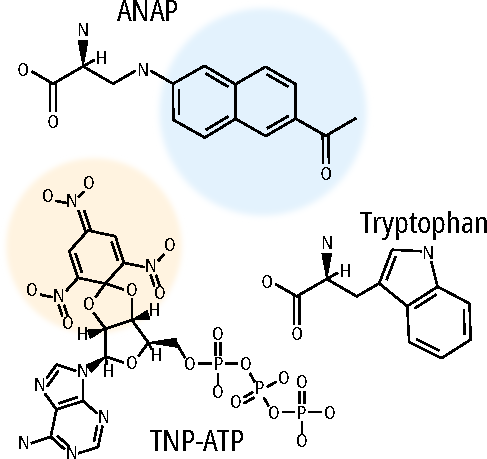
\includegraphics[width=\textwidth]{chemical_structures.pdf}
	\end{subfigure}
	\hfill
	\parbox[t]{0.5\textwidth}{
	\begin{subfigure}[t]{0.5\textwidth}
		\caption{}\label{ch3fig:spectral_overlap}
		\centering
		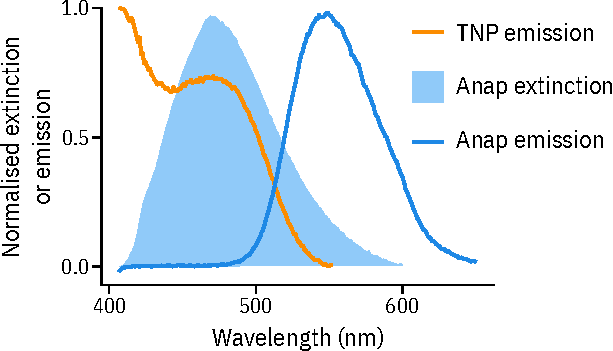
\includegraphics[width=\textwidth]{spectral_overlap.pdf}
	\end{subfigure}
	\hfill
	\begin{subfigure}[t]{0.5\textwidth}
		\caption{}\label{ch3fig:fret_efficiency}
		\centering
		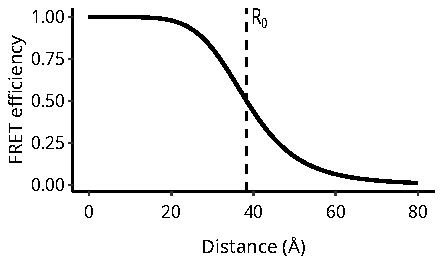
\includegraphics[width=\textwidth]{fret_efficiency.pdf}
	\end{subfigure}
	}
	\caption[Anap and TNP-nucleotides as FRET pairs]{
		\subref{ch3fig:chemical_structures} Chemical structures of Anap and TNP-ATP shown with the fluorescent moieties highlighted in blue (Anap) ot ornage (TNP-ATP).
		\subref{ch3fig:spectral_overlap} Normalised emission spectra (solid lines) of Anap (blue) and TNP-nucleotides (orange) overlayed on the normalised extinction spectra of Anap (filled light blue area).
		Extinction spectra were measured from Anap and TNP-nucleotides alone in aqueous solution.
		Anap emission is the averaged spectra from Kir6.2* + SUR1 expressed in unroofed membranes.
		\subref{ch3fig:fret_efficiency} Theoretical FRET efficiency displayed as a function of the distance between donor and acceptor fluorophores.
		The curve was calculated as a function of the overlap shown in \subref{ch3fig:spectral_overlap}.
		The full formula is discussed in Chapter \ref{ch:2-methods}.
	}

\end{figure}

\subsection{Choosing a site to incorporate ANAP}

THe theoretical R0 of \SI{38.4}{\angstrom} for FRET between ANAP and TNP-ATP allowed for flexibility when choosing a site to incorporate ANAP.
Ideally, a residue should be chosen to maximise the following aims:

\begin{enumerate}
	\item The incorporated ANAP needs to be close enough to the nucleotide binding site of interest to report a quantifiable change in FRET when TNP-ATP is bound.
	This would not have to be close enough for \SI{100}{\percent} FRET to occur, but the greater the efficiency achieved the higher the signal-to-noise ratio would be for measuring binding.
	\item It also needs to be far enough from each other class of nucleotide binding site to avoid quenching by TNP-ATP bound to other sites.
	\item In addition to avoiding interference from other classes of binding site, we also need to avoid cross-talk between nucleotide binding sites of the same class on different subunits, as this would lead to difficulty interpreting the measured quenching.
	The ideal theoretical solution would be labelling only one nucleotide binding site per ion channel, but without using a concatemer this is not so easy in practise.
\end{enumerate}

To narrow down which residues could be candidates for ANAP incorporation to measure binding at Kir6.2, we took three cryo-EM structures of K\ATP{} with ATP bound and computationally docked TNP-ATP into the nucleotide binding pocket (Figure \ref{ch3fig:docking}).
To assess the validity of computationally docking a ligand to each structure, we first attempted to dock ATP to check that the highest-scoring binding poses were similar to those observed in the cryo-EM structures.
Docking ATP to both \#6C3P and \#6C3O yielded binding poses which were very similar to the pose found in the cryo-EM structures (Figures \ref{ch3fig:6c3p_docking}, \ref{ch3fig:6c3o_docking}).
However, docking ATP to \#6BAA resulted in binding poses which were in a flipped orientation relative to the pose found in the cryo-EM structure (Figure \ref{ch3fig:6baa_docking}).

We then took TNP-nucleotide structures from eleven different X-ray diffraction and cryo-EM structures published on RCSB to dock to the Kir6.2 binding site of K\ATP{}.
For both \#6BAA and \#6C3P we observed that the three highest scoring binding poses for TNP-nucleotides closely resemble those of the ATP solved in complex with the channel (Figures \ref{ch3fig:6baa_docking}, \ref{ch3fig:6c3p_docking}).
It is not so clear for \#6C3O, for which the highest scoring poses are not in agreement with each other or the solved structure of ATP.

Based on the predicted TNP-ATP poses for \#6BAA and \#6C3P, we could narrow down potential ANAP incorporation sites to within \SI{25}{\angstrom} of the centre of the TNP-moiety, at which distance we would expect to see over \SI{90}{\percent} FRET efficiency when TNP-ATP is bound to Kir6.2.
In addition, we excluded residues which fell within \SI{45}{\angstrom} of NBS1 or NBS2, as this restricts the potential FRET between TNP-ATP bound at these sites and our chosen residue to roughly \SI{25}{\percent} or less.
While we can exclude residues which fall too close to the NBS's of SUR1, the close proximity of the Kir6.2 nucleotide binding sites to each other means that we cannot exclude intersubunit FRET occuring; i.e. TNP-ATP binding to a neighbouring subunit will also be able to quench ANAP to a certain extent. However, this occurs in a predictable way that we can measure and account for.

We targeted F183 and W311 intitally as they are both bulky hydrophobic residues similar to ANAP, and at which no mutations have been previously identified to alter K\ATP{} function. 

\begin{figure}[h]
	\centering
	\begin{subfigure}[t]{0.28\textwidth}
		\caption{}\label{ch3fig:6baa_docking}
		\centering
		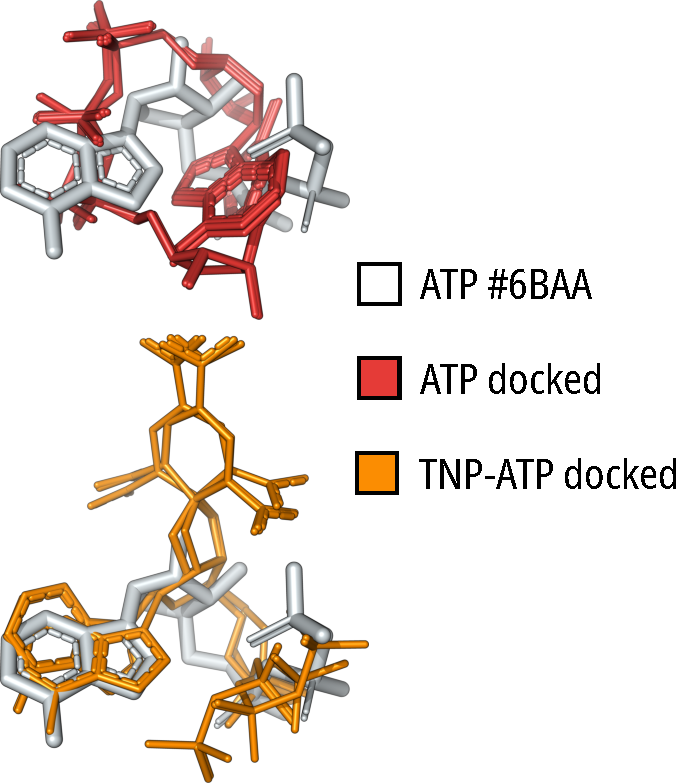
\includegraphics[width=\textwidth]{6baa_docking.pdf}
	\end{subfigure}
	\hfill
	\begin{subfigure}[t]{0.28\textwidth}
		\caption{}\label{ch3fig:6c3p_docking}
		\centering
		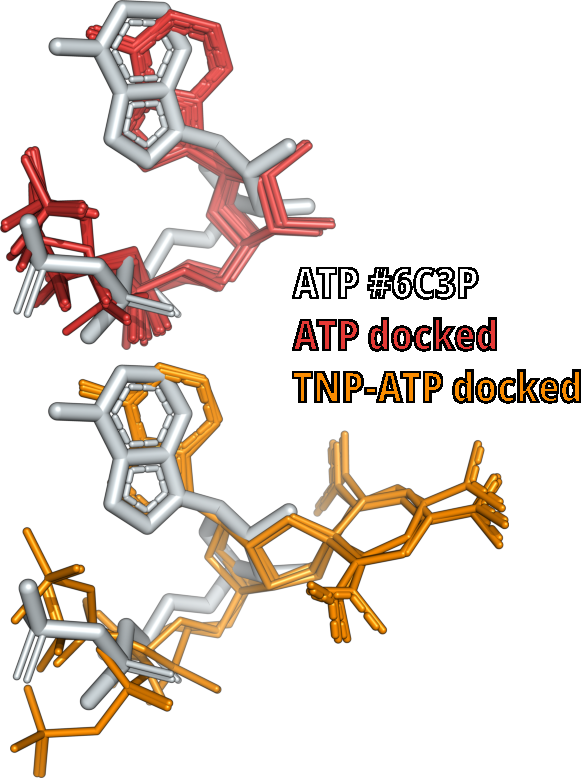
\includegraphics[width=\textwidth]{6c3p_docking.pdf}
	\end{subfigure}
	\hfill
	\begin{subfigure}[t]{0.34\textwidth}
		\caption{}\label{ch3fig:6c3o_docking}
		\centering
		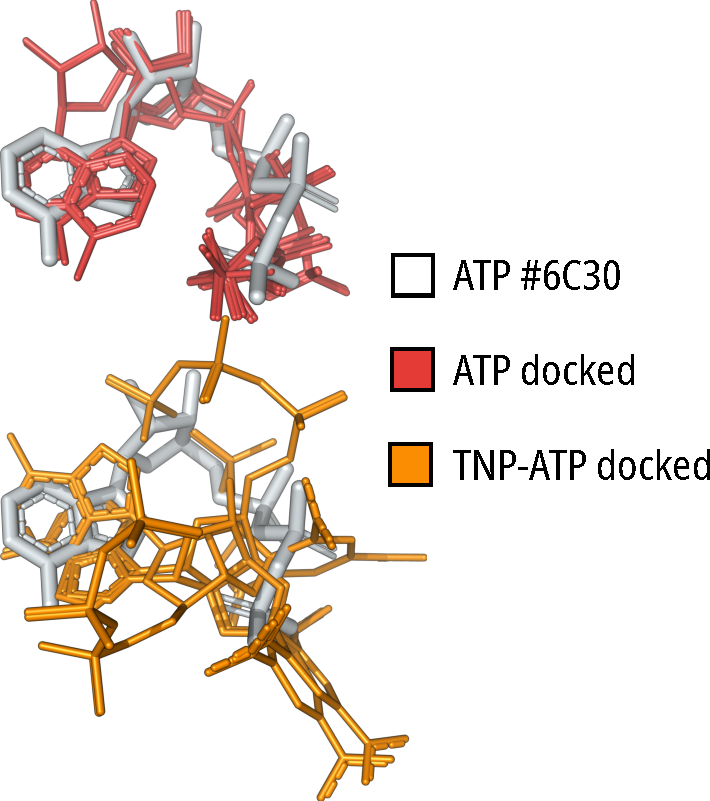
\includegraphics[width=\textwidth]{6c3o_docking.pdf}
	\end{subfigure}
	\vfill
	\begin{subfigure}[t]{0.45\textwidth}
		\caption{}\label{ch3fig:6c3p_bound}
		\centering
		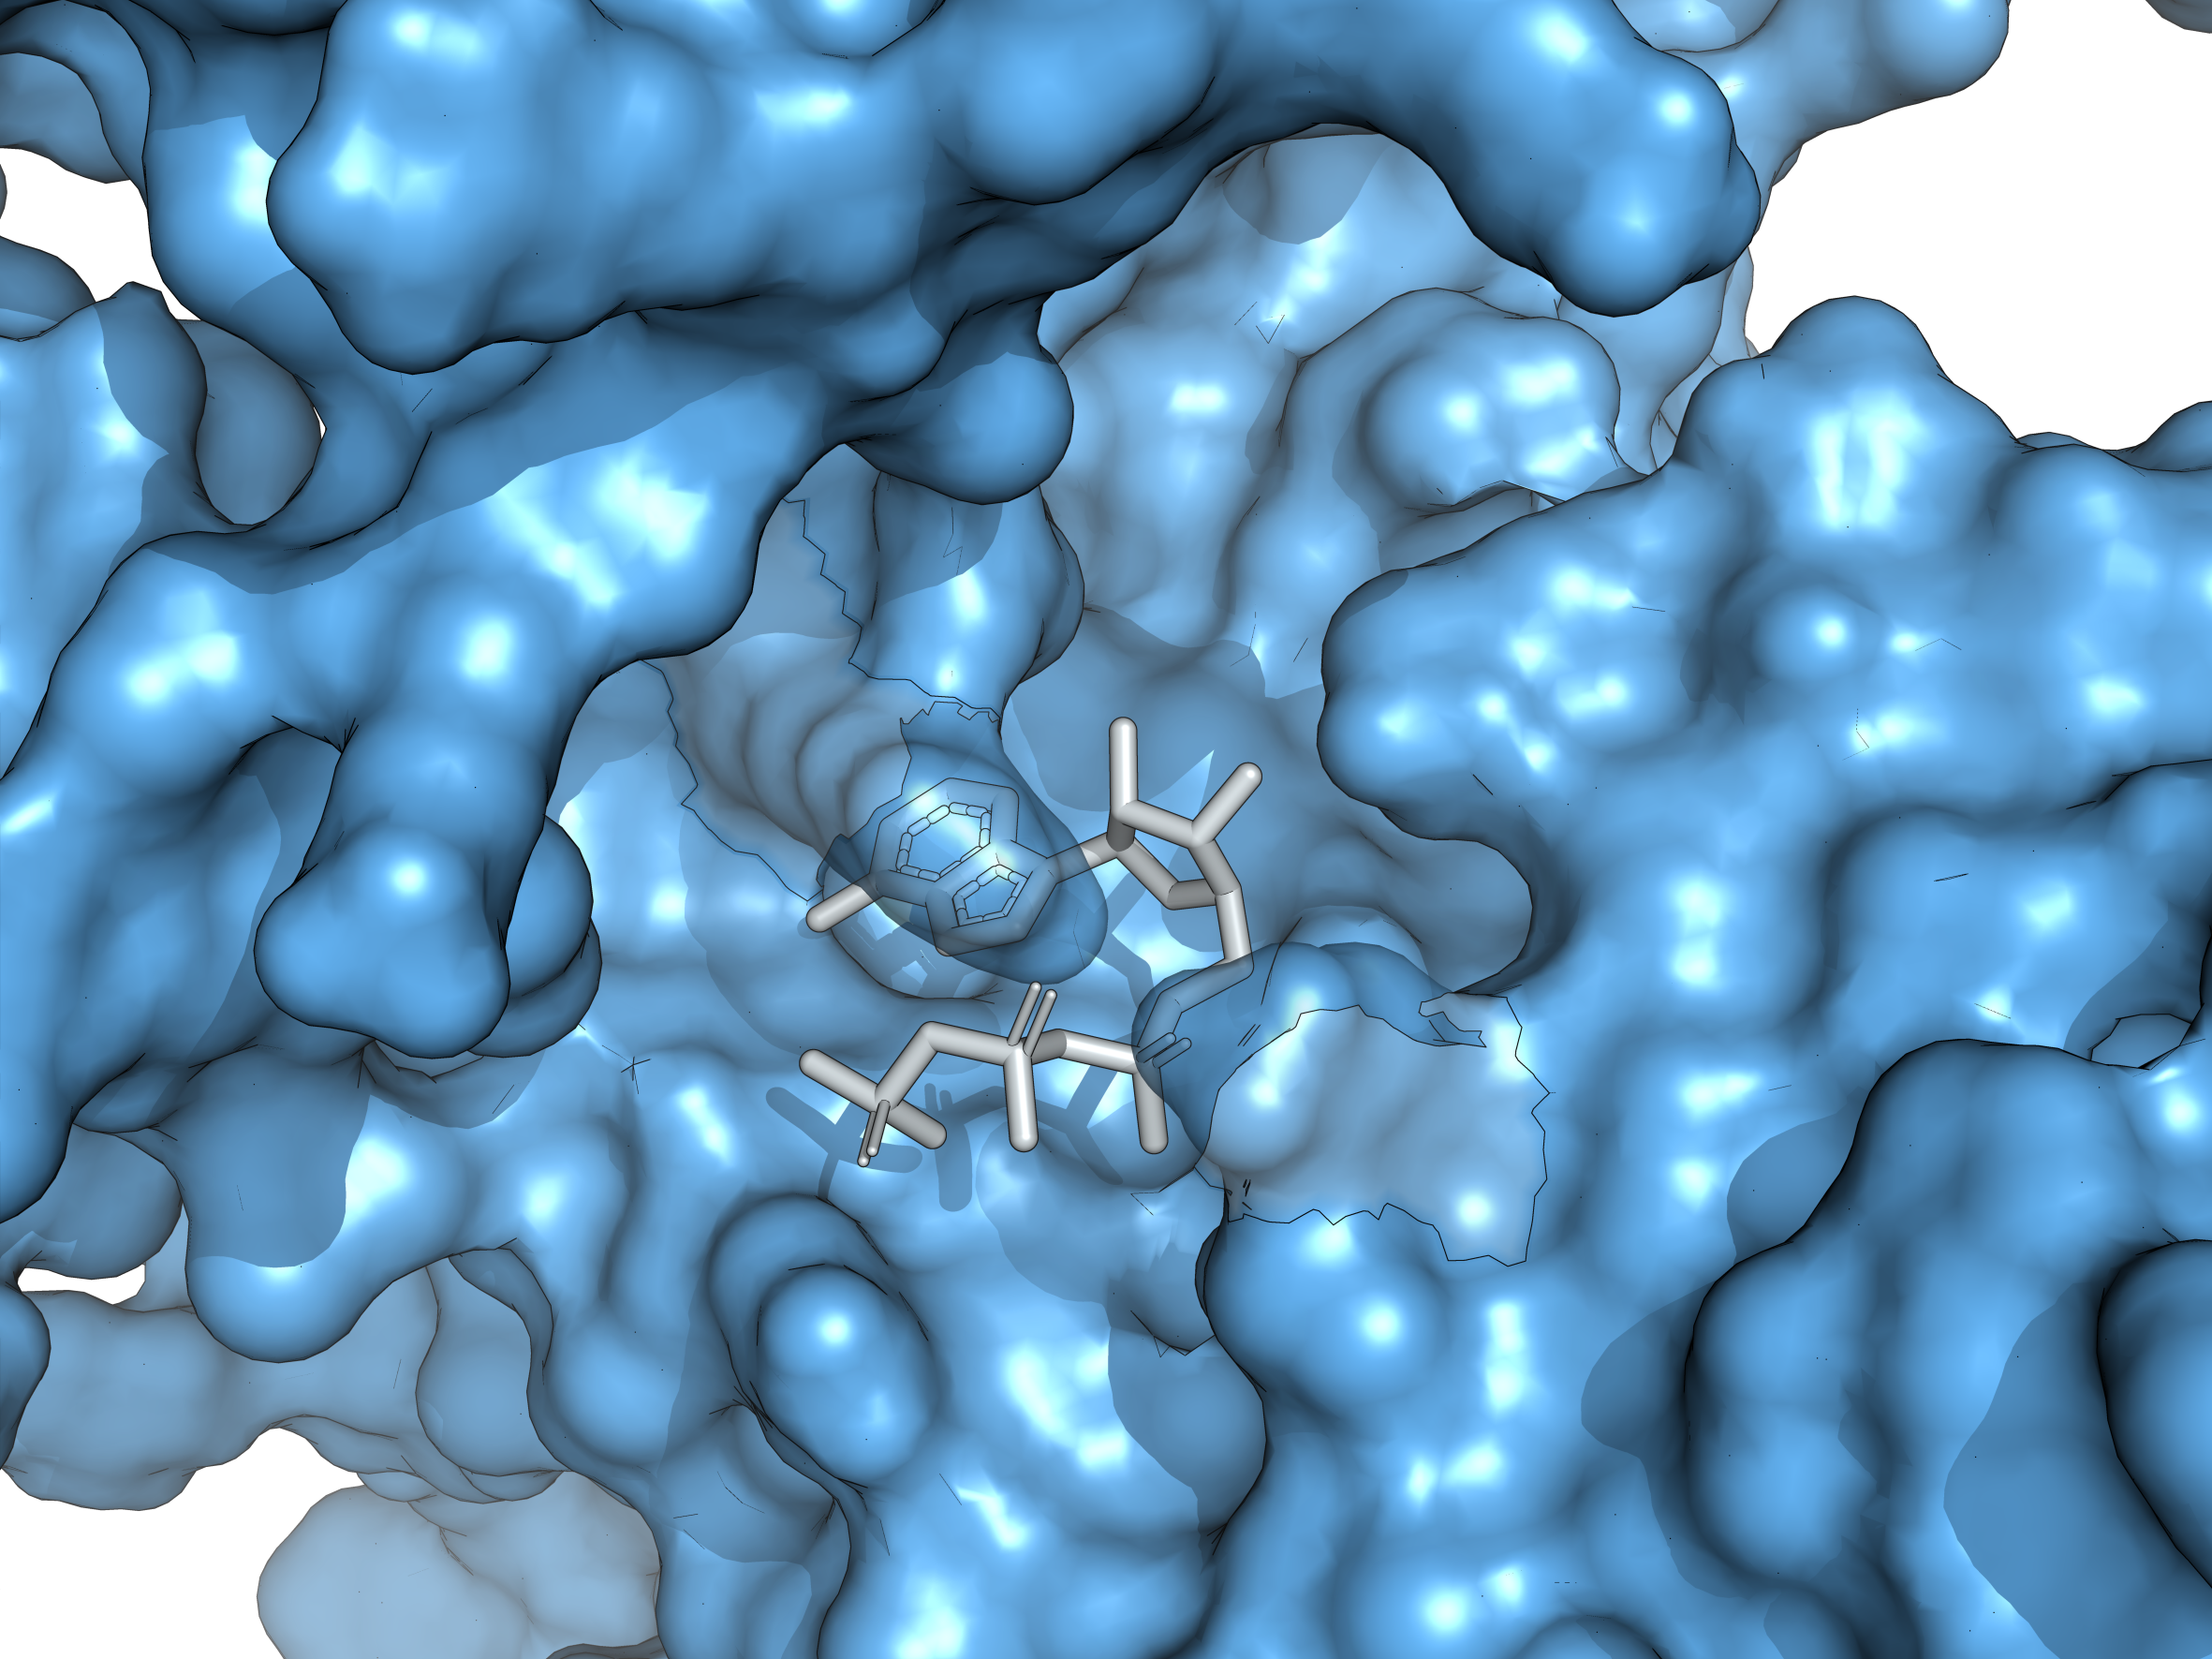
\includegraphics[width=\textwidth]{6c3p_site_bound.png}
	\end{subfigure}
	\hfill
	\begin{subfigure}[t]{0.45\textwidth}
		\caption{}\label{ch3fig:6c3p_docked}
		\centering
		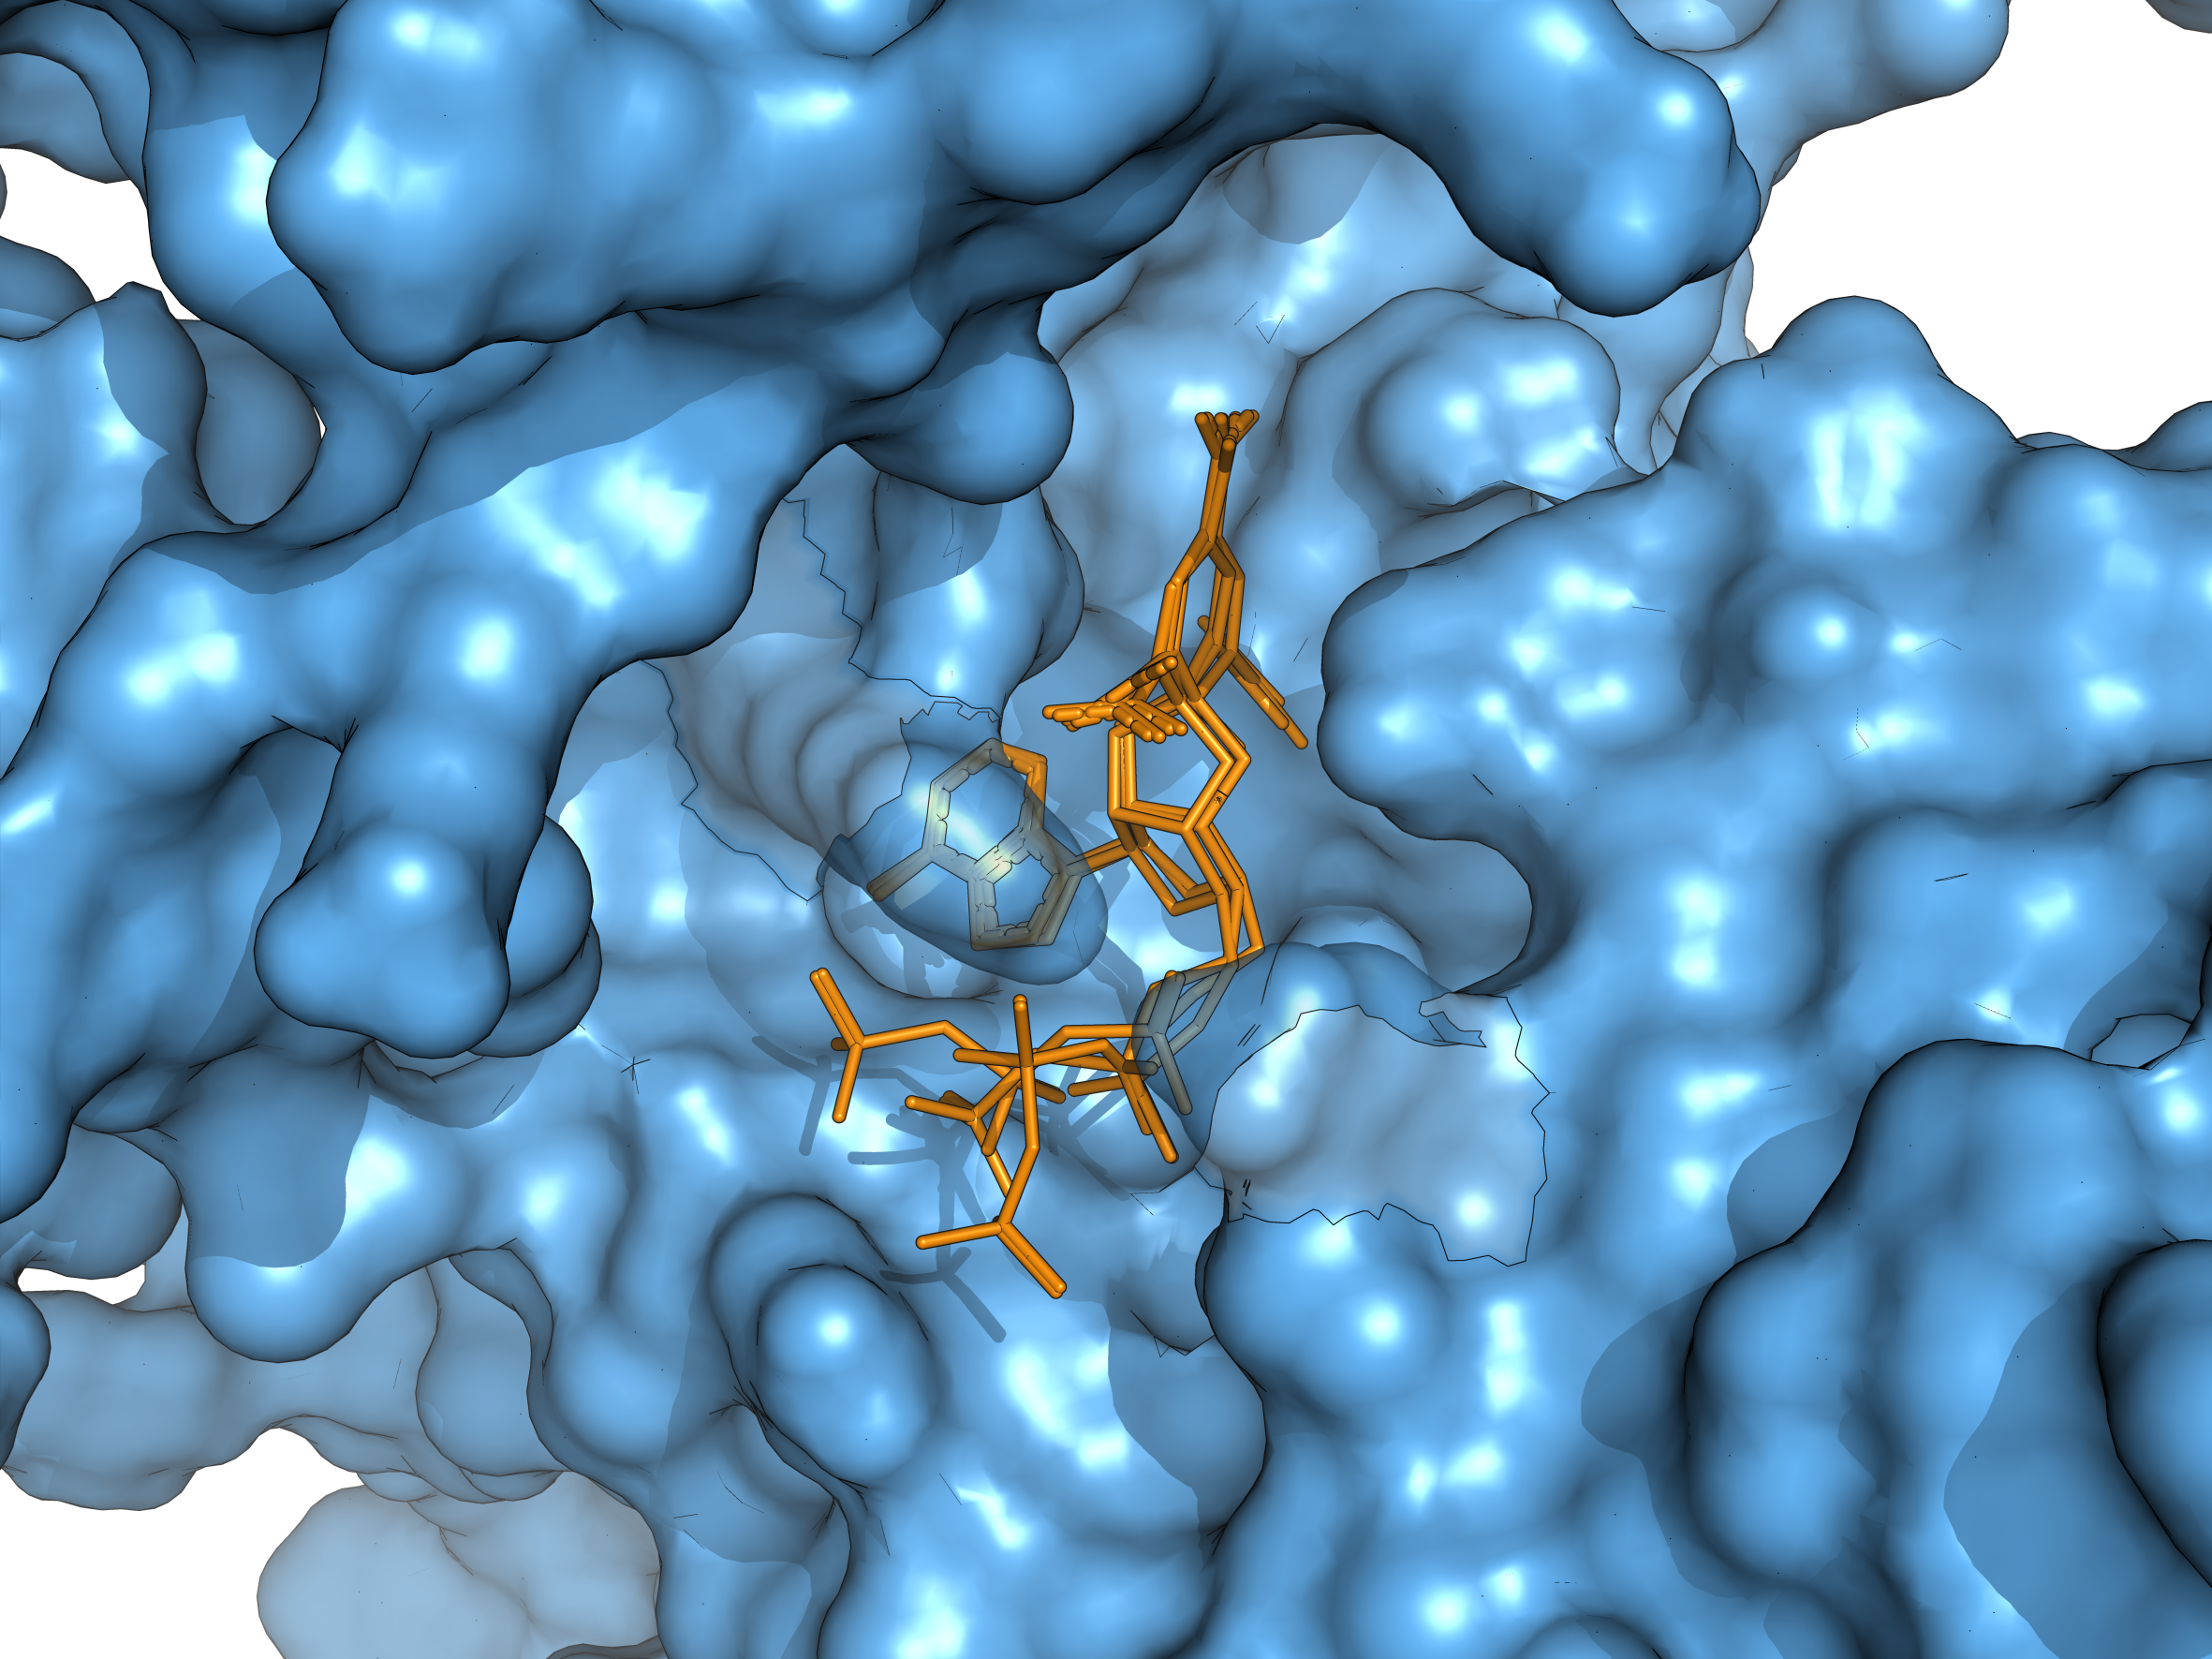
\includegraphics[width=\textwidth]{6c3p_site_docked.png}
	\end{subfigure}
	\caption[TNP-nucleotides can bind with a similar pose to ATP]{
	\subref{ch3fig:6baa_docking}, \subref{ch3fig:6c3p_docking}, \subref{ch3fig:6c3o_docking} Cryo-EM binding poses for ATP bound to Kir6.2 (white) overlayed with either the ten highest scoring computationally docked ATP poses (red) or the three highest scoring computationally docked TNP-nucleotide poses (orange).
	Starting poses for ATP were generated from ten different random seeds based on the cryo-EM poses.
	Starting poses for TNP-nucleotides were generated from eleven structures taken from the RCSB database for different proteins solved in the presence of TNP-ATP.
	The poses shown are from \#3B5J (X-ray diffraction structure of TNP-ADP bound to the NBD complex of a bacterial ABC transporter) and \#5SVQ (X-ray diffraction structure of TNP-ATP bound to the human P2X3 ion channel).
	\subref{ch3fig:6c3p_bound} Cryo-EM structure of the nucleotide binding site in the presence of ATP from \#6C3P.
	\subref{ch3fig:6c3p_docked} As \subref{ch3fig:6c3p_bound} but with the three top scoring binding poses for docked TNP-nucleotides.
	}\label{ch3fig:docking}
\end{figure}

\section{Incorporating ANAP into the Kir6.2 binding site}

\subsection{Amber stop codon expression system}

ANAP can be introduced into a protein of interest by essentially expanding the genetic code to incorporate a noncanconical amino acid.
The amber stop codon (TAG) is the least frequently occuring stop codon in eukaryotic cells, and can be repurposed to encode ANAP.
An orthologous set of tRNA and its aminoacyl-tRNA synthetase are mutated and screened through directed evolution in order to charge the tRNA which recognises the amber stop codon with ANAP.
Thus, in cells expressing the ANAP charged tRNA, the amber stop codon introduced into the protein of interest is suppressed and ANAP is translated instead (Figure \ref{ch3fig:amber_codon}).

\subsection{ANAP incorporation into amber stop codon containing constructs}

\begin{figure}[h]
	\centering
	\begin{subfigure}[t]{0.9\textwidth}
		\caption{}\label{ch3fig:amber_codon}
		\centering
		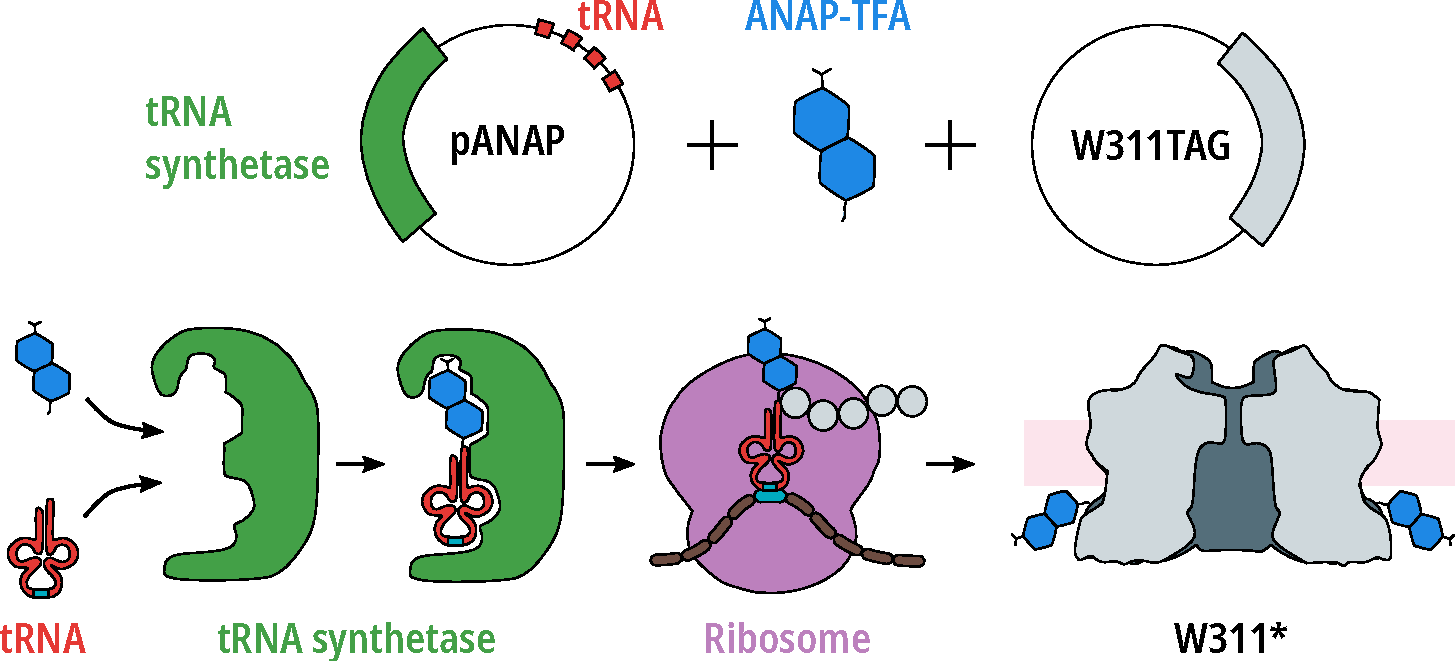
\includegraphics[width=\textwidth]{amber_codon.pdf}
	\end{subfigure}
	\vfill
	\begin{subfigure}[t]{0.45\textwidth}
		\caption{}\label{ch3fig:western_1}
		\centering
		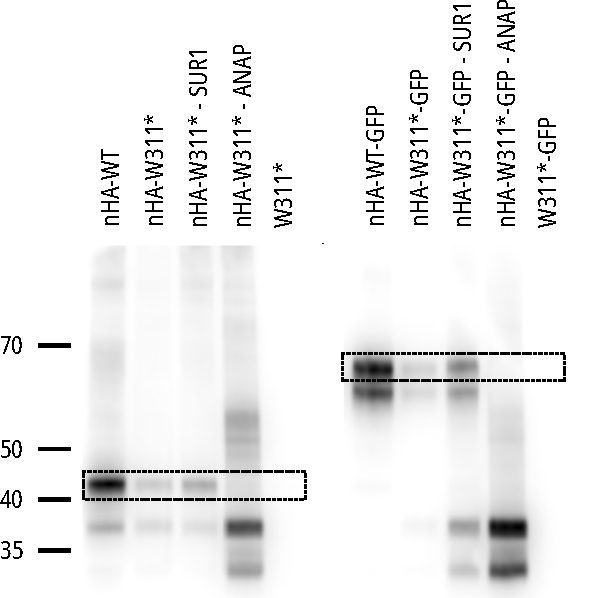
\includegraphics[width=\textwidth]{western_1.pdf}
	\end{subfigure}
	\hfill
	\begin{subfigure}[t]{0.45\textwidth}
		\caption{}\label{ch3fig:western_2}
		\centering
		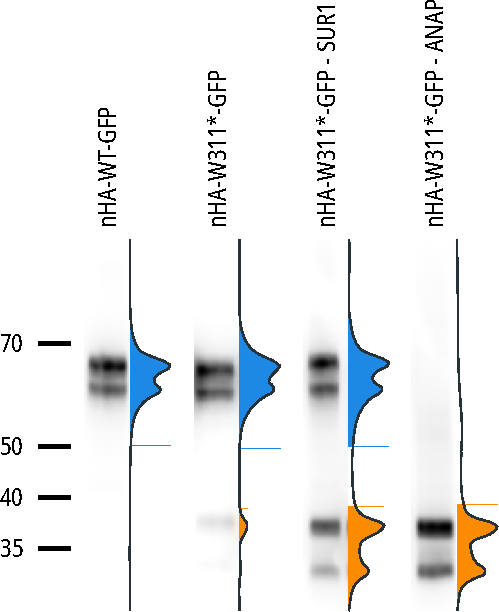
\includegraphics[width=\textwidth]{western_2.pdf}
	\end{subfigure}
	\caption[ANAP incorporation]{
	\subref{ch3fig:amber_codon} ANAP incorporation is accomplished through the transfection of two plasmids.
	pANAP codes for tRNA (red) and it's tRNA synthetase (green), while pW311TAG codes for Kir6.2 with an amber stop codon (TAG) inserted in place of the codon for W311 (grey).
	When the transfected cells are incubated with ANAP (present here as its free acid, ANAP-TFA, blue) the tRNA synthetase assembles tRNA which is capable of recognising the amber stop codon and loads it with ANAP.
	During translation of W311TAG, the primed ANAP tRNAs recognise the TAG and insert ANAP into the desired location.
	\subref{ch3fig:western_1} Two separate western blots against the N-terminal HA epitope incorporated into WT or W311* (left) and WT-GFP or W311*-GFP (right) constructs.
	Cells were co-transfected with pANAP, eRF1-E55D, and SUR1 unless otherwise indicated.
	Full-length Kir6.2 constructs are indicated on each gel with a dashed box.
	The doublets represent an N-terminally truncated product decribed in the main text.
	\subref{ch3fig:western_2} Each lane from the gel containing C-terminally GFP-tagged consstructs is displayed normalised to its highest intensity accompanied by the line averaged density trace.
	The density peak corresponding to full-length Kir6.2 is filled in blue.
	The density peak for C-terminally truncated Kir6.2 is filled in orange.
	}\label{ch3fig:anap_incorporation}
\end{figure}

The nature of the amber stop codon suppression system requires a number of careful controls to ensure the following:

\begin{enumerate}
	\item Stop codon recognition is not perfect, and there is a chance of read-through.
	Instead of incorporating ANAP, it is possible that the translation machinery can insert endogenous amino acids instead, leading to production of full length,unlabelled Kir6.2.
	However, we found that cells transfected with W311TAG constructs and pANAP which were not cultured in the presence of ANAP did not produce full length Kir6.2 (Figure \ref{ch3fig:western_1}, \ref{ch3fig:western_2}), suggesting there is minimal read-through of the stop codon in our experiments.
	\item Introducing a stop codon creates a risk that truncated Kir6.2 will be produced instead of ANAP labelled Kir6.2.
	This risk can be reduced by transfecting a dominant negative engineered version of eukaryotic translation termination factor 1(eRF1-E55D), which does not efficiently terminate protein synthesis in response to the amber stop codon (but leaves opal and ochre stop codons nearly unaffected) and thus increases the incorporation of ANAP.
	We found that transfection of W311TAG constructs with a C-terminal GFP tag produced minimal truncated Kir6.2 (less than \SI{10}{\percent} of the total density observed in Figure \ref{ch3fig:western_2}).
	\item Despite being the least frequent eukaryotic stop codon, the amber stop codon is still present in a significant number of proetin sequences.
	We must be careful that ANAP is not incorporated into a protein which localises to the plasma membrane to an extent which would affect our ability to assign ANAP fluorescence to Kir6.2.
	We found that in cells transfected with GFP-tagged Kir6.2 without an amber stop codon, there was no increase in ANAP fluorescence at the cell membrane (Figure \ref{ch3fig:wt_confocal}, \ref{ch3fig:wt_confocal_profiles}).
	By contrast, when W311TAG-GFP was transfected, we saw a clear increase in ANAP fluorescence at the cell membrane (Figure \ref{ch3fig:w311_confocal}, \ref{ch3fig:w311_confocal_profiles}), suggesting that any observed ANAP fluorescence at the cell membrane originates from our labelled Kir6.2 construct.
\end{enumerate}

\begin{figure}[h]
	\centering
	\begin{subfigure}[t]{0.55\textwidth}
		\caption{}\label{ch3fig:wt_confocal}
		\centering
		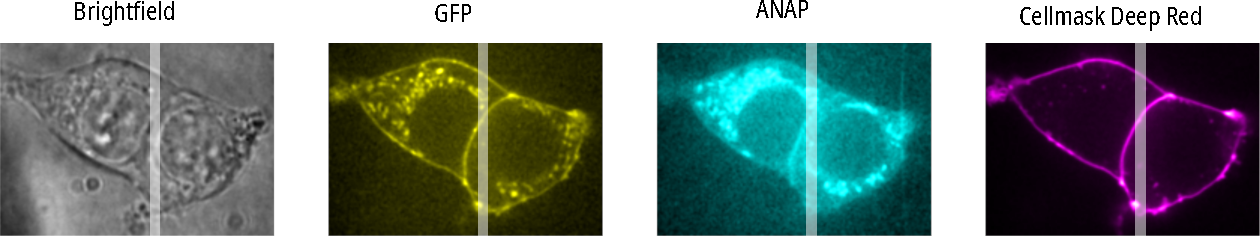
\includegraphics[width=\textwidth]{wt_confocal.pdf}
	\end{subfigure}
	\hfill
	\begin{subfigure}[t]{0.35\textwidth}
		\caption{}\label{ch3fig:wt_confocal_profiles}
		\centering
		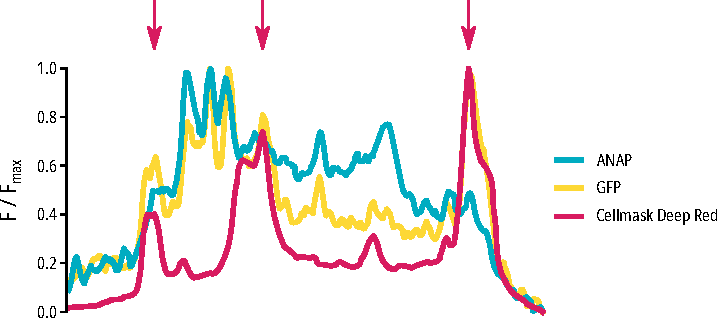
\includegraphics[width=\textwidth]{wt_confocal_profiles.pdf}
	\end{subfigure}
	\vfill
	\begin{subfigure}[t]{0.55\textwidth}
		\caption{}\label{ch3fig:w311_confocal}
		\centering
		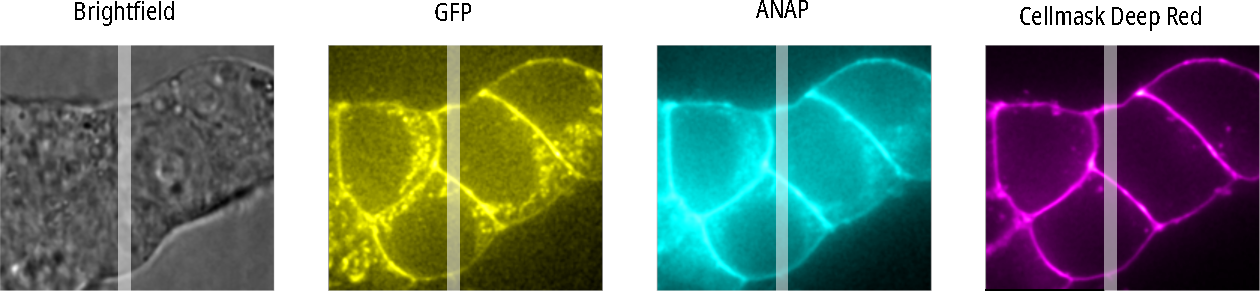
\includegraphics[width=\textwidth]{w311_confocal.pdf}
	\end{subfigure}
	\hfill
	\begin{subfigure}[t]{0.35\textwidth}
		\caption{}\label{ch3fig:w311_confocal_profiles}
		\centering
		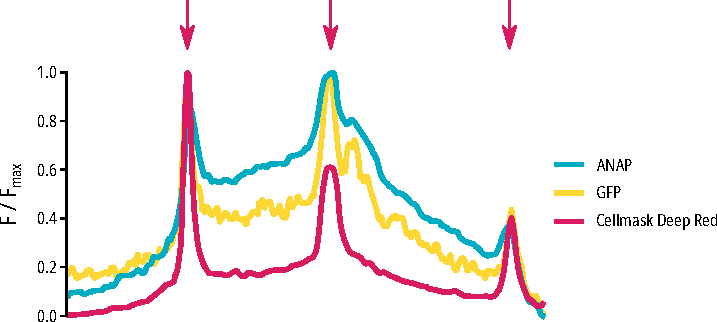
\includegraphics[width=\textwidth]{w311_confocal_profiles.pdf}
	\end{subfigure}
	\caption[Confocal imaging]{
	\subref{ch3fig:wt_confocal}, \subref{ch3fig:w311_confocal} Confocal images of two HEK293T cells transfected with WT-GFP (\subref{ch3fig:wt_confocal}) or W311TAG-GFP (\subref{ch3fig:w311_confocal}), plus SUR1, pANAP, peRF1-E55D and with ANAP in the culture medium.
	Cells were incubated with Cellmask Deep Red for ten minutes before imaging to label the plasma membranes.
	The vertical grey box indicates the section of the images plotted in \subref{ch3fig:wt_confocal_profiles} and \subref{ch3fig:w311_confocal_profiles}
	Images are displayed after median filtering with a box radius of 5, and normalising the intensities per channel.
	\subref{ch3fig:wt_confocal_profiles}, \subref{ch3fig:w311_confocal_profiles}The line-averaged intensity of the pixels in the grey boxes in \subref{ch3fig:wt_confocal} and \subref{ch3fig:w311_confocal} respectively.
	The plasma membranes are identifiable as clear peaks in the Cellmask Deep Red fluorescence (magenta) and are marked with arrows.
	Notably, while there are clear GFP peaks at the membrane in both \subref{ch3fig:wt_confocal_profiles} and \subref{ch3fig:w311_confocal_profiles}, only in \subref{ch3fig:w311_confocal_profiles} do peaks in the ANAP fluorescence coincide with the membrane.
	}
\end{figure}


\section{Testing for functional membrane expression}

\subsection{Surface expression of HA-epitope labelled Kir6.2 constructs}

To assess the ability of ANAP-incorporating constructs to traffic to the plasma membrane, we used a luminence-based surface expression assay.
This assay relies on the recognition of an HA-epitope introduced into an extracellular region of the protein of interest (in this case, the N-terminal region of Kir6.2) by an anti-HA primary antibody followed by an HRP-conjugated secondary antibody.
The luminescence after applying HRP substrate is then proportional to the amount of protein at the plasma membrane of the cells.

We assessed the membrane expression of N-terminally HA-tagged Kir6.2 (nHA-Kir6.2) in the presence or absence of ANAP in the culture media and in the presence or absence of cotransfected SUR1.
We also measured how the addition of a C-terminal GFP tag affected membrane expression under these conditions.
We used untagged Kir6.2 as a control for nonspecific luminesence.

We find that for wild-type Kir6.2 (WT) there is roughly a 20-fold increase in observed luminescence when coexpressed with SUR1 over background, and roughly a 100-fold increase for the C-terminally tagged Kir6.2 (WT-GFP, Figure \ref{ch3fig:surface_expression_1}, \ref{ch3fig:surface_expression_3}).
There is no difference in surface expression of these constructs when ANAP is present in the culture medium (Figure \ref{ch3fig:surface_expression_1}, \ref{ch3fig:surface_expression_4}).
When ANAP is incorporated at either residue 183 or 311 (F183* and W311* respectively) we see an increase in luminescence over background when coexpressed with SUR1 and with ANAP present in the culture medium (Figure \ref{ch3fig:surface_expression_1}, \ref{ch3fig:surface_expression_3}).
The presence of the C-terminal GFP tag increases luminescence further for both constructs, dramatically so for W311*.
However, when F183* is transfected and ANAP is not present in the culture media we still see a similar increase in fluorescence over background when compared to the luminescence when ANAP is present (Figure \ref{ch3fig:surface_expression_1}, \ref{ch3fig:surface_expression_4}), suggesting that a large proportion of the protein reaching the membrane does not have ANAP incorporated.
In contrast, when W311*-GFP is transfected with SUR1 in the presence of ANAP, we see a 10-fold increase in luminescence compared to when ANAP is not present, consitent with the majority of surface expressed protein incorporating ANAP.
We also see a consistent increase in luminescence for all constructs aside from W311* due to cotransfection with SUR1 (Figure \ref{ch3fig:surface_expression_2}), suggesting that the incorporation of ANAP and the addition of a C-terminal GFP tag do not affect the role of SUR1 in froming the full K\ATP{} complex and trafficking to the membrane.

\begin{figure}[h]
	\centering
	\begin{subfigure}[t]{0.45\textwidth}
		\caption{}\label{ch3fig:surface_expression_1}
		\centering
		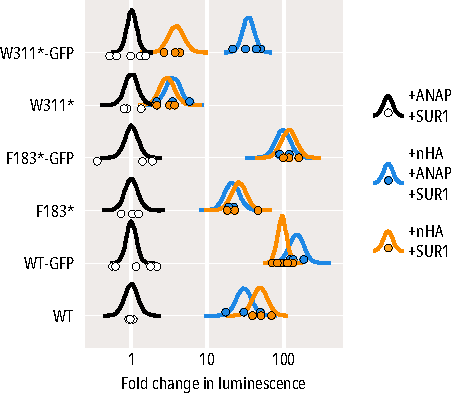
\includegraphics[width=\textwidth]{surface_expression_1.pdf}
	\end{subfigure}
	\hfill
	\begin{subfigure}[t]{0.45\textwidth}
		\caption{}\label{ch3fig:surface_expression_2}
		\centering
		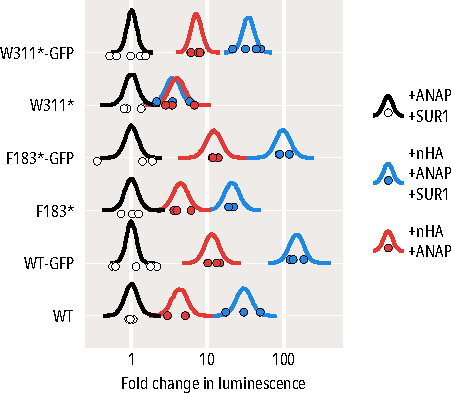
\includegraphics[width=\textwidth]{surface_expression_2.pdf}
	\end{subfigure}
	\vfill
	\begin{subfigure}[t]{0.45\textwidth}
		\caption{}\label{ch3fig:surface_expression_3}
		\centering
		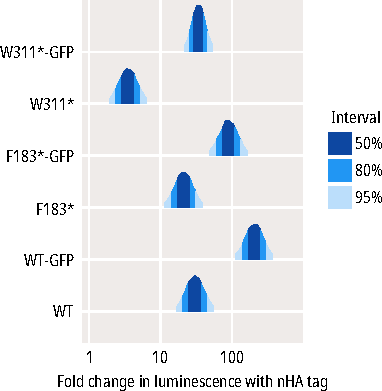
\includegraphics[width=\textwidth]{surface_expression_3.pdf}
	\end{subfigure}
	\hfill
	\begin{subfigure}[t]{0.45\textwidth}
		\caption{}\label{ch3fig:surface_expression_4}
		\centering
		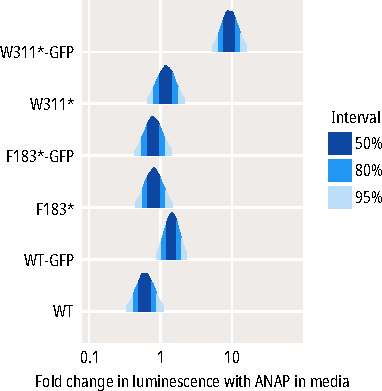
\includegraphics[width=\textwidth]{surface_expression_4.pdf}
	\end{subfigure}
	\caption[ANAP construct surface expression assay]{
	\subref{ch3fig:surface_expression_1}, \subref{ch3fig:surface_expression_2} Individual observations (points) and posterior probability distributions for surface expression of Kir6.2 constructs.
	Before fitting, the observations for each construct were centered by subtracting the mean of the luminesence observed without the N-temrinal HA tag.
	Observations for constructs without the N-terminal HA tag and for constructs transfected with both ANAP and SUR1 are duplicated between panels to clarify the differences observed when either ANAP (\subref{ch3fig:surface_expression_1}) or SUR1 (\subref{ch3fig:surface_expression_2}) are omitted.
	\subref{ch3fig:surface_expression_3}, \subref{ch3fig:surface_expression_4} Contrasts between constructs differing only in the presence or absence of the N-terminal HA-tag (\subref{ch3fig:surface_expression_3}) or the presence or absence of ANAP in the culture media (\subref{ch3fig:surface_expression_4}).
	Different intervals in the posterior probability distribution of the contrasts are shown in shades of blue.
	}
\end{figure}

\subsection{Electrophysiology of Kir6.2 constructs}

To establish whether W311*-GFP formed K\ATP{} channels with similar function to wild-type, we excised patches from cells transfected with either WT-GFP or W311*-GFP cotransfected with SUR1.
Excision was performed in Mg\textsuperscript{2+}-free solution to reduce rundown and to prevent activation of the channel by nucleotides.
We observed similar magnitudes of current for both WT-GFP and W311*-GFP, and currents ran own at similar rates.
Perfusion of ATP resulted in current inhibition with an IC\textsubscript{50} of x for WT-GFP and x for W311*-GFP.
Thus, despite the distance from the ATP binding site, the W311 mutation clearly affects some aspect of nucleotide inhibition.
However, we assume that insights into the function of the ANAP-incorporating channel will still be applicable to wild-type channels despite the change in nucleotide inhibition.

Next, we established that TNP-ATP inhibits K\ATP{} to a similar extent as ATP.
We observed current inhibition with an IC\textsubscript{50} of x for WT-GFP and x for W311*-GFP.
K\ATP{} thus appears to be more sensitive to inhibition by TNP-ATP than by ATP.
This could potentially be due to extra contacts made by the TNP moiety with Kir6.2, seen in our computational docking.
Despite the change in the relative IC\textsubscript{50}, there is nothing that would suggest a different mechanism of action for TNP-ATP inhibition.

\subsection{Unroofed membrane binding assay of Kir6.2 constructs}

We then directly measured nucleotide binding to W311*-GFP in unroofed membranes.
Briefly sonicating transfected cells adhered to coverslips results in the lower membrane of the cell remaining stuck to the coverslip while the rest of the cell contents is disrupted and perfused away.
This leaves the cytoplasmic domains of expressed K\ATP{} channels open to perfusion of TNP-ATP.
By measuring the fluorescence spectra of patches of unroofed membrane, we can separate the fluorescence emission peaks of the C-terminal GFP tag and the incorporated ANAP.

Perfusing TNP-ATP results in a decrease in the peak corresponding to ANAP fluorescence, and a concomittant increase in a fluorescence peak which corresponds to the TNP-ATP.
This phenomenon is the fresult of FRET between TNP-ATP bound to the channel at the Kir6.2 binding site.
The decrease in ANAP fluorescence is almost directly correlated to an increase in bound nucleotide.

To equivocate ANAP quenching and nucleotide binding, first we need to correct for incomplete FRET due to the distance between the donor and acceptor.
Based on the computational docking, we predicted a maximal FRET efficiency of \SI{95}{\percent} when every Kir6.2 subunit is bound by TNP-ATP.
Fitting our observed data to a Hill equation results in a maximum observed FRET efficiency of \SI{93}{\percent}, agreeing well with our prediction.
We can then normalise our observed fluorescence data by this value.

Secondly, we need to adjust for the FRET between adjacent subunits of Kir6.2.
The difference between the ideal 1:1 subunit/ligand FRET efficiency and the simulated experimental FRET efficiency resulted in a correction factor of $log_2(\frac{F}{F_{max}} + 1)$.
Overall, these two corrections do not dramatically alter our results, and we performed our analysis on both corrected and uncorrected results to ensure that there was no potential difference in interpration which derived from treating our data in this way.

We observed quenching of ANAP fluorescence over a concentration range of TNP-ATP similar to the range in which we observed inhibition of current in W311*-GFP.
When fit to a Hill equation, quenching was fit with an EC\textsubscript{50} of x, while the corrected binding data gave an EC\textsubscript{50} of x.
Notably, this EC\textsubscript{50} is somewhat right-shifted compared to the IC\textsubscript{50} we observed in excised patches (x).

\subsection{Patch-clamp fluorometry of Kir6.2 constructs}

To ensure that the ANAP fluorescence we observe in the unroofed membranes is emitted by functional channels, and thus the quenching by TNP-ATP reflects nucleotide binding to the same population of channels we are measuring inhibition from, we measured fluorescence quenching and current inhibition from the same excised patches.

This experimental paradigm leads to two complications compared to performing the measurements separately.
Firstly, the number of channels in an excised patch are far smaller than the number of channels in an unroofed membrane patch.
This results in a much dimmer fluorescence readout, and a lower signal-to-noise ratio.
Secondly, the presence of the pipette glass in the images results in some abnormalities in the background subtraction procedure.
This is not due to the glass itself, but results from the occlusion of TNP-ATP from the image surrounding the patch.
This leads to oversubtraction of the background TNP-ATP spectra, leading to an apparent negative peak in our corrected images.
However, we find that there is no overlap of this peak and the ANAP peak, so our fluorescence quenching measurements are unaffected by this phenomenon.

Our fluoresence measurements from excised patches agree reasonably well with our measurements for unroofed membranes.
Our finding that the EC\textsubscript{50} for TNP-ATP binding is right-shifted compared to the IC\textsubscript{50} for TNP-ATP inhibition is consistent between each experimental paradigm.
This finding has implications for how exactly the binding of nucleotides to Kir6.2 leads to closure of the K\ATP{} channel pore.

\begin{figure}[h]
	\centering
	\begin{subfigure}[t]{0.9\textwidth}
		\caption{}\label{ch3fig:atp_tnpatp_trace}
		\centering
		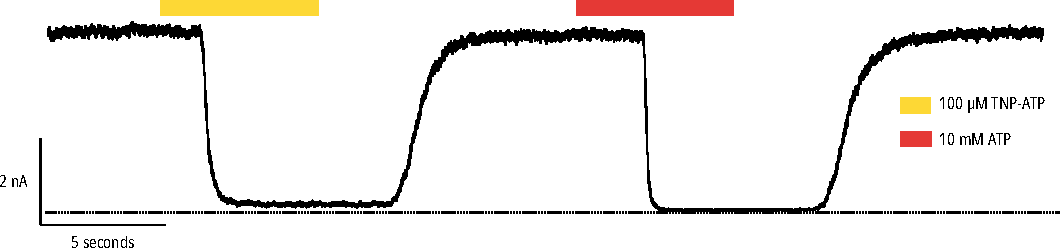
\includegraphics[width=\textwidth]{atp_tnpatp_trace.pdf}
	\end{subfigure}
	\vfill
	\begin{subfigure}[t]{0.5\textwidth}
		\caption{}\label{ch3fig:atp_tnpatp_spectra_1}
		\centering
		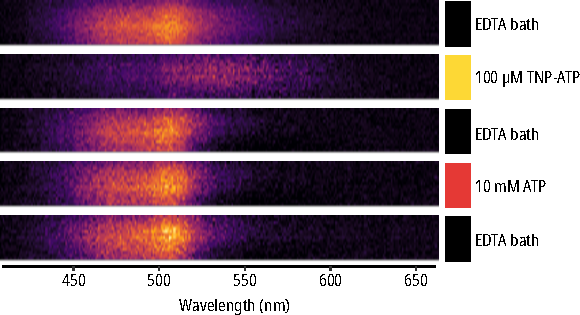
\includegraphics[width=\textwidth]{atp_tnpatp_spectral_images.pdf}
	\end{subfigure}
	\hfill
	\begin{subfigure}[t]{0.4\textwidth}
		\caption{}\label{ch3fig:atp_tnpatp_spectra_2}
		\centering
		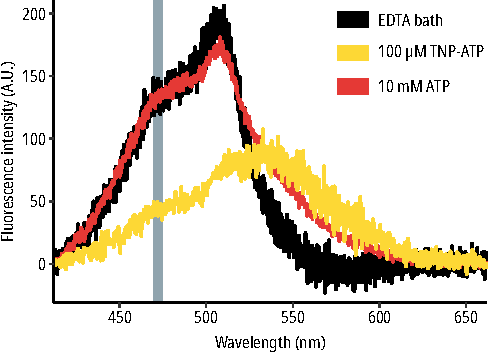
\includegraphics[width=\textwidth]{atp_tnpatp_spectral_traces.pdf}
	\end{subfigure}
	\caption[ANAP is not quenched by ATP]{
	\subref{ch3fig:atp_tnpatp_trace} Current trace from an excised patch expressing W311*-GFP+SUR1 perfused with either ATP or TNP-ATP.
	The zero current level is shown as a dotted line, and the nucleotide applications are marked as coloured bars.
	\subref{ch3fig:atp_tnpatp_spectra_1} Spectra captured from the same patch during the nucleotide applications marked in \subref{ch3fig:atp_tnpatp_trace}, and during the washout periods between applications.
	Each spectra was captured with a one second exposure and corrected for background fluorescence and bleaching as described elsewhere.
	\subref{ch3fig:atp_tnpatp_spectra_2} Averaged traces of the spectra shown in \subref{ch3fig:atp_tnpatp_spectra_1}. The location of the peak ANAP fluorescence is marked by a grey box.
	}
\end{figure}


\subsection{Scanning a region}

Introduced cutting sites and pasted in oligos
(with Mike and Tascia - Mike did the molecular biology on SUR, I did on Kir6.2, Mike and I did surface expression together, Tascia did ephys on the mutants that expressed).
